\documentclass[20pt,margin=1in,innermargin=-3.5in,blockverticalspace=-0.25in]{tikzposter}
\geometry{paperwidth=40in,paperheight=30in}
\usepackage[utf8]{inputenc}
\usepackage{amsmath}
\usepackage{amsfonts}
\usepackage{amsthm}
\usepackage{amssymb}
\usepackage{mathrsfs}
\usepackage{graphicx}
\usepackage{adjustbox}
\usepackage{enumitem}
\usepackage[backend=biber,style=numeric]{biblatex}
\usepackage{emory-theme}
\usepackage{url}
\usepackage{hyperref}
\usepackage{mwe} % for placeholder images

% set theme parameters
\tikzposterlatexaffectionproofoff
\usetheme{EmoryTheme}
\usecolorstyle{EmoryStyle}

\title{Retrospective of Gamma Function}
\author{Liangzho Lin 40085480}
\institute{ {Repository: \url{https://github.com/linliangzhao/soen6011.git}}}



% begin document
\begin{document}
\maketitle
\centering
\begin{columns}
    \column{0.5}
    \block{Critical Decisions}{
 \textbf{\Large I made three important decisions throughout the project.}
 \section{Algorithm selection}
There are two algorithms for calculating gamma function, one is Lanczos algorithm and the other is Stirling algorithm. It is a very important decision to decide to choose Lanczos algorithm in this project.
\newline
As shown in Figure 1, The accuracy of the Stirling algorithm increases with increasing x, but the accuracy in the interval of 0-0.5 is very low, which is a disadvantage that cannot be optimized.
\begin{tikzfigure}[\large Comparison of Stirling's approximation with the factorial.]
            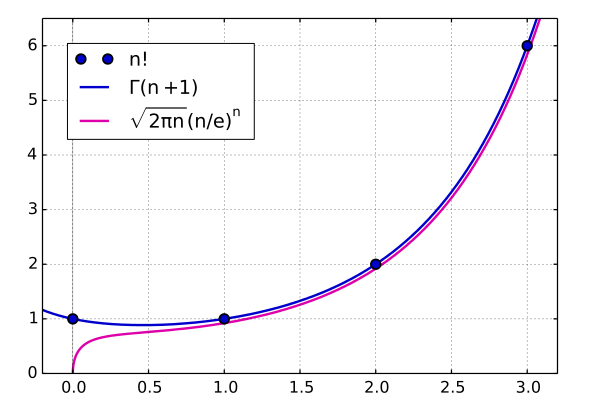
\includegraphics[width=0.3\linewidth]{figure2.png}
        \end{tikzfigure}
However, as for Lanczos algorithm,The accuracy of the calculation results increases as levels of expansion of the series increases. I made the formula progresses to the 6th level series, which makes the result of the function accurate to the six decimal places accurate, so that the accuracy of my function satisfies the requirements of the project.
\section{Two formulas are added to improve the algorithm}
Since the Lanczos algorithm can only compute cases where x is greater than 1, in order to be able to calculate x less than 1, I have optimized the function's method. I added the recursion formula  $\Gamma \left( x \right) = \frac{\Gamma \left( x +1\right)}{x}$ and the reflection formula $\frac{\pi }{\Gamma \left( 1-x \right)\sin(\pi x)}$ according to the characteristics of the gamma function.
\newline
The recursion formula converts inputs less than 1 into inputs greater than 1 by recursion so that the input can still be calculated by the Lanczos algorithm.
\newline
However, if the user's input is a negative number with large absolute values, it will cause too many recursive times, causing a long calculation time or even a stack overflow error. 
\newline I add the reflection formula so the function avoids excessive recursion, which improves efficiency and security. This is a good decision.
\section{Direct output “Infinity" for input less than $-10^8$}
According to the characteristics of the image of the gamma function (as shown in Figure 2), the value of $\Gamma \left( x \right)$ when $x$ is less than $-10^8$ can be directly considered as infinity.
\begin{tikzfigure}[\large Gamma Function. ]
            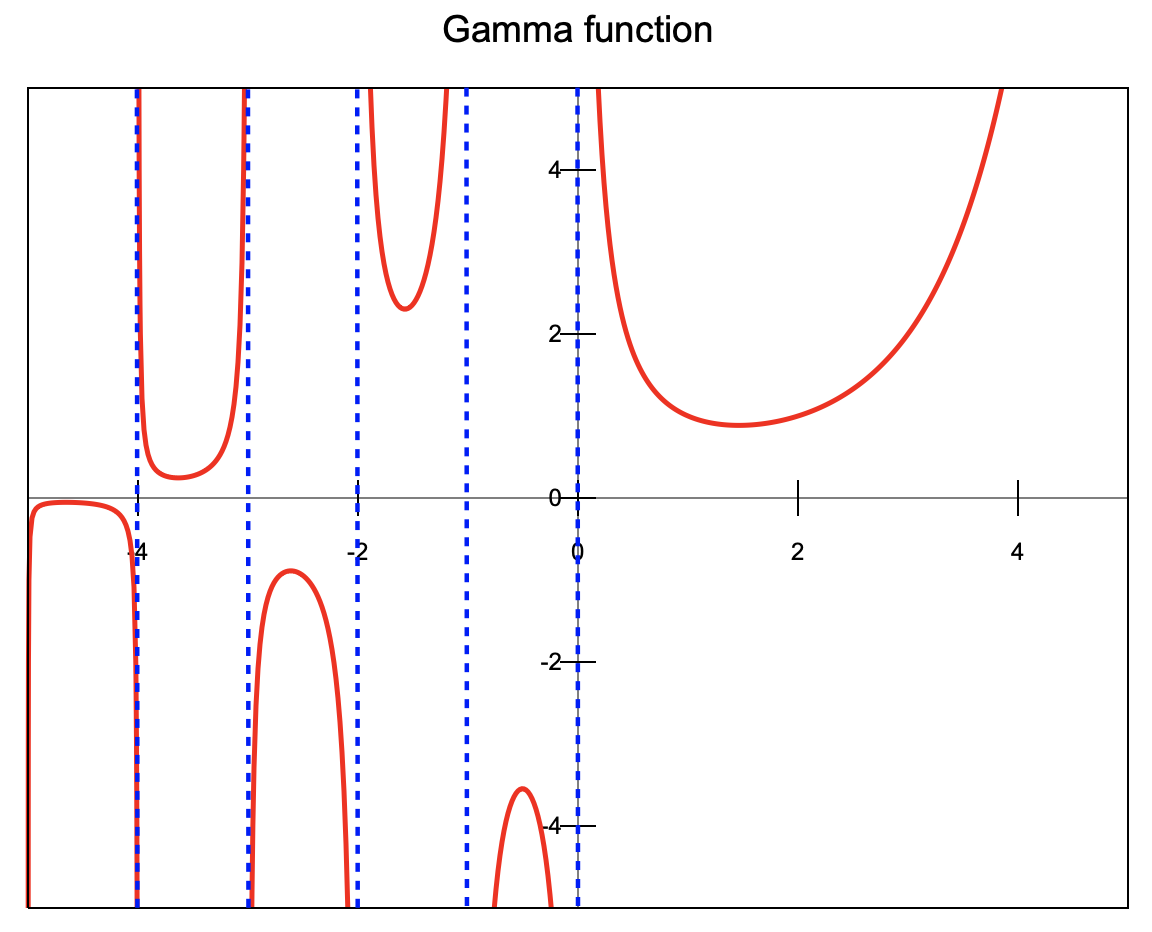
\includegraphics[width=0.3\linewidth]{gammafunction.png}
        \end{tikzfigure}
If the input less than $-10^8$ is calculated by the algorithm, the calculation time will be very long and all the result are infinity.Therefore, I decided to identify the input less than $-10^8$ in the process of input identification and directly output infinite without entering the algorithm to calculate, thus improving efficiency.
    }

    \column{0.5}
    \block{Lessons Learnt}
    {
 \textbf{\Huge General}
 \newline
  \newline
  \LARGE{
Through this project, I noticed that the entire complete system not only pays attention to the functional requirements, but also pays attention to the non-functional requirements. These non-functional requirements can increase the value of the entire project.}
 \newline
  \newline
 \textbf{\Huge Experience gained through team review}
 \newline
  \newline
  \LARGE{
According to my teammates' feedback on the code review, I feel that I should do a better job in programming style. Try to avoid redundant code during the project and avoid resigning parameters in each math function. This, in turn, can avoid confusion and improve the maintainability of my project.}
 \newline
  \newline
 \textbf{\Huge Experience gained through testing}
 \newline
  \newline
  \LARGE{All my test cases have been successfully passed in my teammate's test. The experience of this project allowed me to learn to use JUnit's framework to write and run test cases for the project.  
  \newline
  At the beginning, when I tested the project, I needed to run the program once per test case, which was a waste of time. With JUnit, I can test all test cases in one execution. What's more, structure of the test cases is standardized so that all testers can know at a glance which method will be tested and know the test result very soon. Therefore, in future projects, I will also use JUnit for testing.}

    }
    \block{Reference}{\LARGE{\noindent[1] C. Lanczos, "A precision approximation of the gamma function," Journal of the Society for Industrial and Applied Mathematics, Series B: Numerical Analysis, vol. 1, (1), pp. 86-96, 1964.
\newline
[2] H. Robbins, "A remark on Stirling's formula," The American Mathematical Monthly, vol. 62, (1), pp. 26-29, 1955.
\newline
[3] P. J. Davis, "Leonhard Euler's integral: A historical profile of the Gamma function: In memoriam: Milton Abramowitz," The American Mathematical Monthly, vol. 66, (10), pp. 849-869, 1959. }}
\end{columns}
\end{document}